\documentclass[a4paper,14pt]{extreport}
\usepackage[utf8]{inputenc}
\usepackage[T2A]{fontenc}
\usepackage[russian]{babel}
\usepackage{eufrak}
% поля:
\usepackage[left=1cm, right=1cm, top=2cm, bottom=2cm]{geometry}
\linespread{1}
\usepackage{indentfirst} % отделять первую строку раздела абзацным отступом
\setlength\parindent{5ex}
\addto{\captionsrussian}{\renewcommand*{\contentsname}{Содержание}}
\usepackage[hidelinks]{hyperref} % гиперссылки в содержании
\usepackage{graphicx}
\usepackage{float}
\usepackage{amsmath}
\renewcommand*{\thesection}{\arabic{section}}

\usepackage{multirow}
\usepackage[normalem]{ulem}
\useunder{\uline}{\ul}{}

\usepackage{cmap}%позволяет копировать кириллицу из скомпилированного файла

% Глубина разделов, попадающих в содержание
\setcounter{tocdepth}{3}

\linespread{1.3} % настройка межстрочного интервала
\tolerance=1000 % настройка чувствительности вставки переносов
\hfuzz=0pt
\sloppy

\begin{document}
	
	\begin{titlepage}
		\begin{center}
			\large
			МИНИСТЕРСТВО ОБРАЗОВАНИЯ И НАУКИ\\ РОССИЙСКОЙ ФЕДЕРАЦИИ
			
			\textbf{Федеральное агентство по образованию}
			\vspace{0.5cm}
			
			УНИВЕРСИТЕТ ИТМО
			\vspace{0.25cm}
			
			Факультет компьютерных технологий и управления
			
			Кафедра систем управления и информатики
			\vfill
			
			
			Студент: Артемов Кирилл\\
			группа P4135\\
			Вариант №2\\
			\textsc{Лабораторная работа №4}\\[5mm]
			
			{\LARGE Синтез дискретных стабилизирующих алгоритмов управления}
			\bigskip
			
		\end{center}
		\vfill
		
		\newlength{\ML}
		\settowidth{\ML}{«\underline{\hspace{0.7cm}}» \underline{\hspace{2cm}}}
		\hfill\begin{minipage}{0.4\textwidth}
			Преподаватель\\
			\underline{\hspace{\ML}} Ю.\,В.~Литвинов\\
			«\underline{\hspace{0.7cm}}» \underline{\hspace{2cm}} 2016 г.
		\end{minipage}%
		\bigskip
		
		\vfill
		
		\begin{center}
			Санкт-Петербург, 2016 г.
		\end{center}
	\end{titlepage}
	\newpage
	
	\section{Цель работы}
	
	Ознакомление с принципами синтеза дискретных регуляторов систем автоматического управления, работающих в режиме стабилизации.
	
	\section{Вариант задания}
	
	\begin{table}[H]
		\centering
		\caption{Параметры ОУ}
		\label{my-label}
		\begin{tabular}{|c|c|c|c|c|c|c|c|c|c|}
			\hline
			№ & ОУ & $k_1$ & $a_0^1$ & $T_1$ & $\xi$ & $k_2$ & $a_0^2$ & $T_2$ & T   \\ \hline
			2 & 1  & 1     & 0       & 0     & 0     & 0.5   & 1       & 0.95  & 0.5 \\ \hline
		\end{tabular}
	\end{table}
	
	\begin{figure}[H]
		\center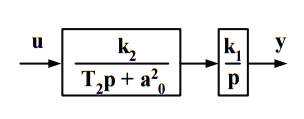
\includegraphics[width=0.5\linewidth]{oc.png}
		\caption{Объект управления}
		\label{fig:scr1}
	\end{figure}
	
	\section{Порядок выполнения работы}
	
	1. Получение модели ВСВ для непрерывного объекта.
	
	Модель «Вход-состояние-выход» непрерывного объекта управления описывается уравнениями:
	\begin{equation}
	\begin{cases}
	\dot x(t) &= A x(t) + B u(t)\\
	y(t) &= C x(t)
	\end{cases}
	\end{equation}
	
	Подставив параметры ОУ из таблицы 1 в ОУ на рисунке 1, получим:
	\begin{equation}
	W(p) = \frac{k_1 k_2}{T_2 p^2 + a_0^2 p} = \frac{0.5}{0.95 p^2 + p} 
	\end{equation}
	
	Перейдем к канонической управляемой форме.
	
	Для начала приведем передаточную функцию к виду с единичным старшим коэффициентом полинома.
	
	\begin{equation}
	W(p) = \frac{\frac{k_1 k_2}{T_2}}{p^2 + \frac{a_0^2}{T_2} p} = \frac{0.5263}{p^2 + 1.0526  p} 
	\end{equation}
	
	Теперь приведем к канонически управляемой форме:
	
	\begin{equation}
	A=
	\begin{bmatrix}
	0&1\\
	0& 1.0526
	\end{bmatrix}
	\end{equation}
	\begin{equation}
	B=
	\begin{bmatrix}
	0\\
	0.5263
	\end{bmatrix}
	\end{equation}
	\begin{equation}
	C=
	\begin{bmatrix}
	1&0
	\end{bmatrix}
	\end{equation}
	
	2. Переход к дискретному описанию объекта управления.
	Дискретные системы в пространстве состояний описываются разностными уравнениями.
	\begin{equation}
	\begin{cases}
	x(k+1) &= A_d x(k) + B_d u(k)\\
	y(k) &= C x(k)
	\end{cases}
	\end{equation}
	
	Из таблицы 1 интервал дискретности $T = 0.5$ сек.
	Матрицы $A_d, B_d$ рассчитаем в среде моделирования Scilab.
	\begin{figure}[H]
		\center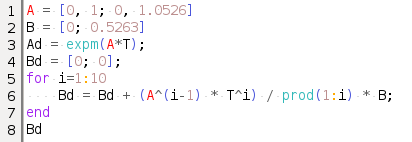
\includegraphics[width=0.5\linewidth]{adbd.png}
		\caption{Листинг программы расчета матриц $A_d, B_d$}
		\label{fig:scr1}
	\end{figure}
	В результате получим следующие матрицы:
	\begin{equation}
	A_d=
	\begin{bmatrix}
	0&0.2859793\\
	0& 1.3010219
	\end{bmatrix}
	\end{equation}
	\begin{equation}
	B_d=
	\begin{bmatrix}
	0.0179897\\
	0.1505109
	\end{bmatrix}
	\end{equation}
	
	3. Моделирование непрерывного и дискретного объекта управления
	
	\begin{figure}[H]
		\center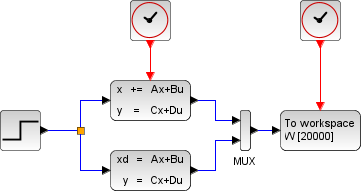
\includegraphics[width=0.5\linewidth]{model_1.png}
		\caption{Схема моделирования ОУ}
		\label{fig:scr1}
	\end{figure}
	
	\begin{figure}[H]
		\center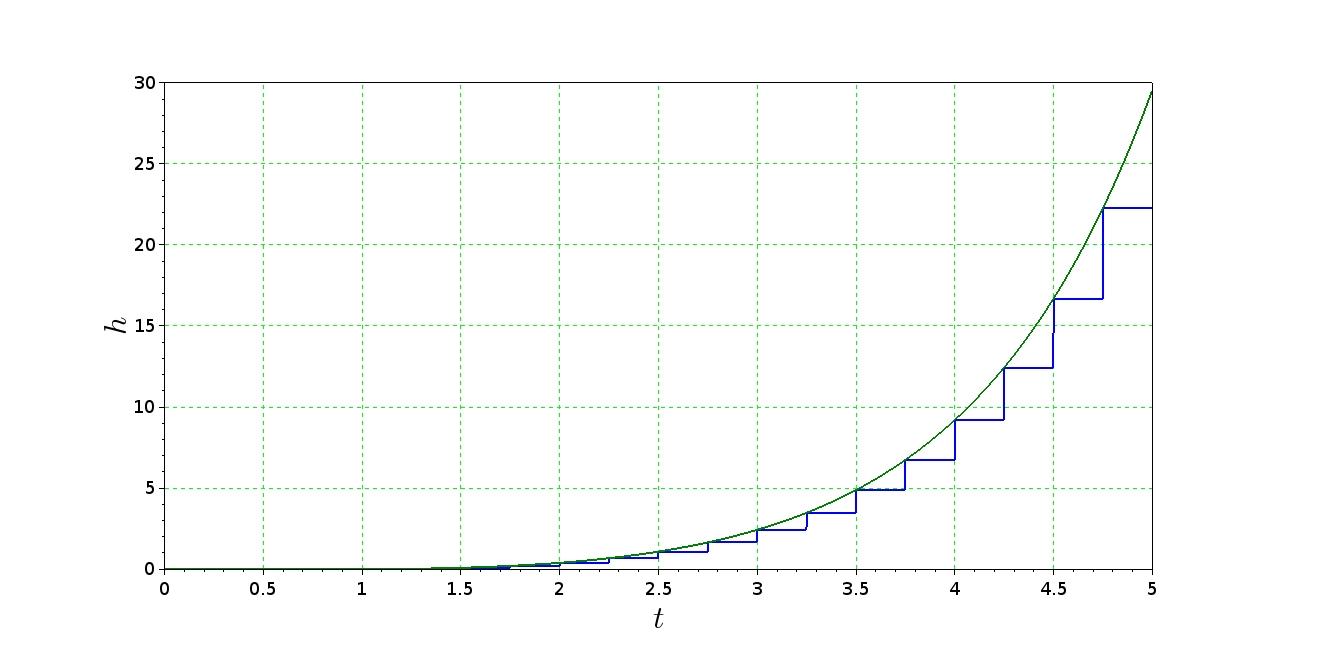
\includegraphics[width=0.7\linewidth]{model_1_res.png}
		\caption{Результаты моделирования ОУ}
		\label{fig:scr1}
	\end{figure}
	
	4. Вывод о преобразовании ОУ.
	
	Как видно из рисунка 4, дискретная модель точно описывает непрерывную, экстраполирую сигнал в моменты $t = kT = 0.5k$, где $k = 1..n$.
	
	5. Анализ дискретного объекта.
	
	— на полную управляемость;
	
	Для анализа системы на управляемость строится матрица следующего вида:
	\begin{equation}
	U_d =
	\begin{bmatrix}
	B_d & Ad B_d & \dots & A_d^{n-1} B_d
	\end{bmatrix}
	\end{equation}
	
	Если определитель матрицы управляемости не вырожден $det(U_d) \ne 0$, можно полагать, что пара матриц $A_d, B_d$ -- полностью управляема.
	
	Для рассчитанного ранее ОУ, определитель матрица управляемости равен:
	\begin{equation}
	U_d =det
	\begin{bmatrix}
	0.0179897    &0.0610327  \\
	0.1505109    &0.1958180
	\end{bmatrix}
	=- 0.0056634  \ne 0
	\end{equation}
	Из чего заключаем, что система полностью управляема.
	
	— на полную наблюдаемость.
	
	Для анализа системы на наблюдаемость строится матрица следующего вида:
	\begin{equation}
	Q_d =
	\begin{bmatrix}
	C_d\\
	C_d A_d\\
	\vdots\\
	
	C_d A_d^{n-1}
	\end{bmatrix}
	\end{equation}
	
	Если матрица наблюдаемости не вырождена, то объект полностью наблюдаем.
	
	Для рассчитанного ранее ОУ, определитель матрица наблюдаемости равен:
	\begin{equation}
	Q_d =det
	\begin{bmatrix}
	1&    0\\         
	1 &   0.2859793  
	\end{bmatrix}
	=0.2859793  \ne 0
	\end{equation}
	Из чего заключаем, что система полностью наблюдаема.
	
	— на устойчивость.
	Для анализа устойчивости найдем корни характеристического полинома дискретного ОУ. Воспользуемся функцией $spec(Ad)$, чтобы найти собственные числа матрицы.
	
	\begin{align}
	z_1 &= 1. \\ 
	z_2 &= 1.3010219  
	\end{align}
	
	Так как $z_i > 0$, следовательно, ОУ не устойчивый в соответствии с
	корневым критерием.
	
	6. Построение эталонной модели для корней оптимальной дискретной системы по быстродействию, то есть $z_i = 0$ при $i = 1,...,n$.
	
	Сформируем эталонную модель вида:
	\begin{equation}
	\begin{cases}
	\xi(k+1) = \Gamma_d \xi(k)\\
	y(k) = H_d \xi(k)
	\end{cases}
	\end{equation}
	где $\xi(k)$ -- вектор состояния дискретной эталонной модели, матрицы $\Gamma_d, H_d$ строятся в соответствии с требуемыми показателями качества.
	
	Составим следующие матрицы:
	\begin{equation}
	\Gamma_d = 
	\begin{bmatrix}
	z & 1\\
	0 & z
	\end{bmatrix}
	=
	\begin{bmatrix}
	0 & 1\\
	0 & 0
	\end{bmatrix}
	\end{equation}
	\begin{equation}
	H_d = 
	\begin{bmatrix}
	1&0&0& \dots &0
	\end{bmatrix}
	=
	\begin{bmatrix}
	1 & 0
	\end{bmatrix}
	\end{equation}
	
	7. Найти матрицу линейных стационарных обратных связей.
	
	Определим эталонный характеристический полином.
	\begin{equation}
	D^*(z) = det[zI - \Gamma_d] = det
	\begin{bmatrix}
	z & -1\\
	0 & z
	\end{bmatrix}
	= z^2
	\end{equation}
	
	Характеристический полином с матрицей состояния дискретной системы имеет вид:
	
	\begin{equation}
	D(z) = det[zI - A_d] = z^2 - 2.6926579z + 1.6926579  
	\end{equation}
	\begin{equation}
	k_{i+1}^k = a_i^* - a_i
	\end{equation}
	\begin{equation}
	K^k = 
	\begin{bmatrix}
	k_1^k & k_2^k
	\end{bmatrix}
	\end{equation}
	где $a_i^*$ -- коэффициенты полинома эталонной модели, $a_i$ -- коэффициенты полинома ОУ.
	
	\begin{align}
	k_1^k = a_0^* - a_0 = 0 - 1.6926579 = - 1.6926579\\
	k_2^k = a_1^* - a_1 = 0 + 2.6926579  = 2.6926579\\
	\end{align}
	
	В результате проделанных действий получим матрицу линейных стационарных обратных связей в канонически управляемом базисе:
	\begin{equation}
	K^k = 
	\begin{bmatrix}
	- 1.6926579 & 2.6926579
	\end{bmatrix}
	\end{equation}
	
	Теперь перейдем в исходный базис.
	\begin{equation}
	K_d = K^k M^{-1}
	\end{equation}
	где $M = U_d U_k^{-1}$ -- матрица преобразования.
	$U_k$ -- матрица наблюдаемости, сформированная парой матриц $A_k, B_k$, принадлежащих канонической управляемой форме ОУ.
	
	Сформируем матрицы $A_k, B_k$:
	\begin{equation}
	A_k =
	\begin{bmatrix}
	0 & 1\\
	-1.6926579 & 2.6926579
	\end{bmatrix}
	\end{equation}
	\begin{equation}
	B_k = \begin{bmatrix}
	0\\
	1
	\end{bmatrix}
	\end{equation}
	
	Сформируем матрицу управляемости для канонической управляемой формы ОУ:
	\begin{equation}
	U_k =det
	\begin{bmatrix}
	0&1\\
	1&2.6926579
	\end{bmatrix}
	=- 1  \ne 0
	\end{equation}
	
	Теперь, найдем $M$:
	\begin{equation}
	M = U_d U_k^{-1} =
	\begin{bmatrix}
	0.0941421  &  0.0790224  \\
	- 0.3463289   & 0.3463289  
	\end{bmatrix}
	\end{equation}
	
	Применяя полученное значение матрицы преобразования $M$, определим МЛСОС в первоначальном базисе:
	\begin{equation}
	K_d = 
	\begin{bmatrix}
	5.7748572    &6.4571995 
	\end{bmatrix}
	\end{equation}
	
	8. Проведем моделирование замкнутой системы при начальных условиях $y(0) = 1, \dot y(0) = 0$.
	\begin{figure}[H]
		\center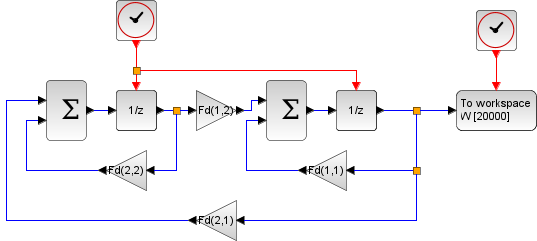
\includegraphics[width=0.7\linewidth]{model_fd.png}
		\caption{Схема моделирования замкнутой системы}
		\label{fig:scr1}
	\end{figure}
	\begin{figure}[H]
		\center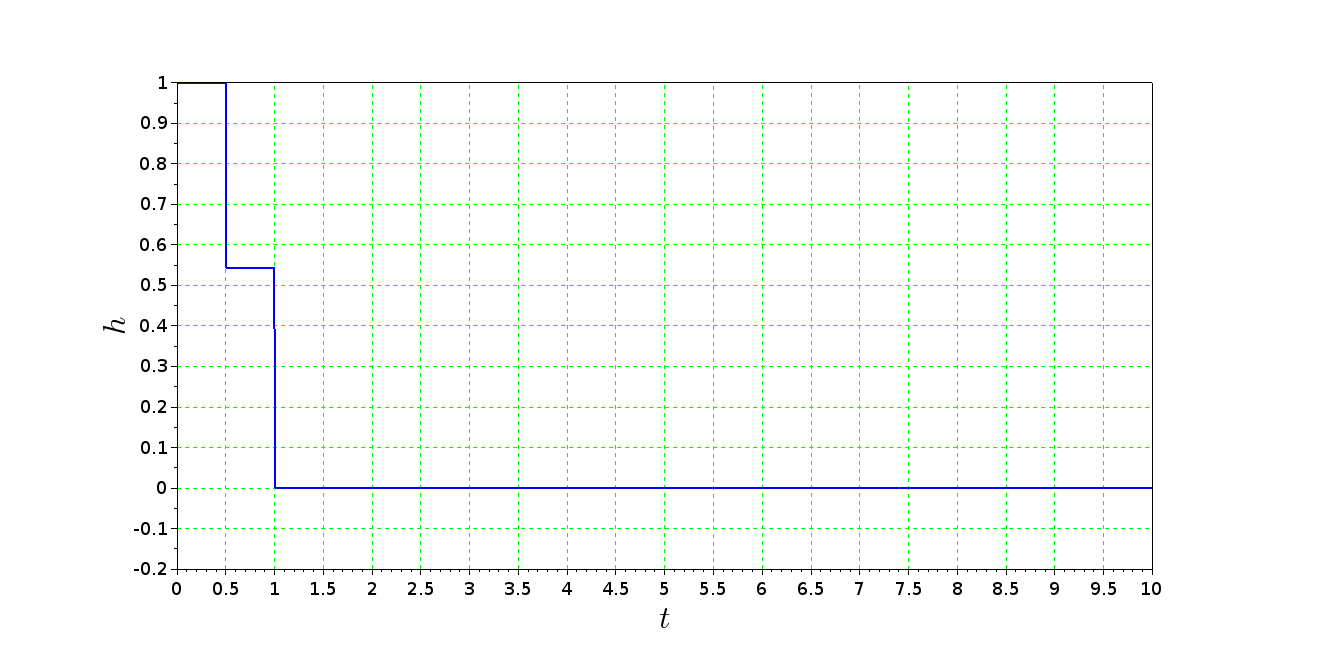
\includegraphics[width=0.7\linewidth]{model_fd_res.png}
		\caption{Результаты моделирования замкнутой системы}
		\label{fig:scr1}
	\end{figure}
	
	9. Вывод о соответствии результатов моделирования и
	желаемого поведения.
	
	Как видно из рисунка 6, полученная модель системы соответствует
	желаемому поведению системы: стабилизируется в устойчивом положении.
	Также, полученная система является оптимальной по быстродействию, так как выполняется услвие:
	\begin{align}
	t_n \le nT\\
	1 sec. = 2 * 0.5 sec.
	\end{align}
	где $t_n$ -- время переходного процесса, $n = 2$ -- порядок системы, $T = 0.5$ --
	интервал дискретности.
	
\end{document}
